\RequirePackage{fix-cm}
%
%\documentclass{svjour3}                     % onecolumn (standard format)
%\documentclass[smallcondensed]{svjour3}     % onecolumn (ditto)
%\documentclass[smallextended]{svjour3}       % onecolumn (second format)
\documentclass[twocolumn]{svjour3}          % twocolumn
\smartqed  % flush right qed marks, e.g. at end of proof
\usepackage{graphicx}
\usepackage[linesnumbered,ruled,vlined]{algorithm2e}
\usepackage{tabularx}
\journalname{CGI2013} % The correct name will be entered by the editor
\begin{document}

\title{Cloth and Avatar Preparation for Virtual Fitting Rooms } 
\subtitle{Preprocessing approach for real-time virtual fitting room with physics simulation}
\author{Umut Gultepe  \and Ugur Gudukbay}
\institute{Bilkent University \at Ankara \and Bilkent University \at Ankara}
\date{ }% The correct dates will be entered by the editor

\maketitle

\begin{abstract}
This paper presents a novel approach to adjusting a virtual cloth and avatar with respect to a specific user for a virtual fitting room framework. Proposed method scales the cloth and the avatar accordingly with the subjects body dimensions, also prepares the physics simulation and collision detection environment, with a total preprocessing time of one second, eliminating the requirement for long preprocessing times to achieve a realistic fitting experience.
\keywords{Virtual Fitting Room \and Depth Sensor \and Character Animation}
\end{abstract}

\section{Introduction}
\label{sec:1}
Apparel industry is one of the biggest on the planet, estimated to be \$2,560 trillion worldwide in 2010 \cite{Breyer2012}. It is also the second biggest and fastest growing e-commerce sector \cite{Fredricksen2012}. One of the most time-consuming stages of apparel shopping is trying the apparels on, which is not even possible in online stores. With the advances in the augmented reality technologies, virtual fitting rooms are slowly taking their places in both real and virtual stores  \cite{Fitnect2012,Styku2013} to imrpove the quality of apparel trying experience while also making it faster.

Advanced virtual fitting rooms show the apparel items either on the video of the user or on a virtual avatar, both scaled to reflect the user's body characteristics \cite{FaceCake2013}. Some of them also employ physics based garment simulation for a better fitting experience\cite{Styku2013}.

This paper presents a new approach to adjusting a virtual clothing item and a virtual avatar for a specific subject on the fly. Constraining the overall preprocessing time to 1 second, the clothing piece and the avatar is adjusted automatically and prepared for a physics powered virtual fitting room framework. 

\section{Previous Works}
\label{sec:2}
Virtual fitting rooms have been a research subject for more than a decade. Protopsaltou \cite{Protopsaltou2002} has developed an internet based approach for virtual fitting rooms, although it was not real time and required marker based motion capture systems for animation. Zhang \cite{Zhang2008} used a multi-camera system utilizing SFS \cite{Cheung2005} techniques to build a real time intelligent fitting room. 

Advances in time-of-flight technology made depth sensors available at consumer-level prices with better performance. This prompted a wave of research based on depth sensors in various fields, such as Rehabilitation \cite{Yao2011}, indoor modeling \cite{Peter2012} and medicine \cite{Gallo2012}. Another topic which attracted significant attention from both researchers and companies is real-time virtual fitting rooms. Giovanni \cite{Giovanni2012} developed a virtual try-on system utilizing a calibrated set of Kinect and an HD Camera, while comparing the two state of the art depth sensing SDKs- OpenNI\cite{OpenNI2013} and Kinect for Windows SDK\cite{Microsoft2013}.

One problem every researcher encountered during their studies with depth sensors is the feeble quality and noisiness of the depth stream. This problem is analyzed in depth by Khoshelham \cite{Khoshelham2012} and concluded that standard deviation reaches 2cm in a measuring distance of 3m. Matyunin \cite{Matyunin2011} attempted to improve the quality by filtering with additional information from the attached RGB camera.  

\section{Methodology}
\label{sec:3}
Objective is to acquire a set of simulation parameters from a human test-subject for a pre-modeled clothing mesh, which is to be displayed on a virtual avatar reflecting the body characteristics of the aforementioned subject.  The set of parameters for the simulation include the body height and width, also the radii for the collision  spheres which have their centers coinciding with the joints of the virtual avatar's skeleton.
Body width and height are then utilized to estimate the body size of the user, collision spheres are used in the dressing room simulation, to collide with the cloth particles.   
  
\subsection{Depth Map Optimization}
\label{subsec:3.1} 
The state-of the art time-of-flight cameras still provide low resolution and quality output compared to current advanced RGB systems. The quality of the input depth map is a crucial factor on the overall performance of the system, therefore we first wish to improve the quality of the depth map by applying canonical image optimization methods.

In this approach, we assume utilization of a time-of-flight camera running with a middleware which also provides a subject map, which has the same size as and denotes the origin of the pixels of the depth map, either belonging to a subject or to the background.

Let us take the input depth map D as a MxN matrix. Initially, the user pixels from D are extracted by a pixel-by-pixel comparison with the input user map. We are only interested in the one subject and $D_1$ represents the depth pixels of him, whereas $U_1$ is the bit map of the subject. Also, the non-subject pixels are set to the mean value of the user pixels, to set the matrix properly for the subsequent optimizations.

\begin{equation}
D_1=(D-(D \times U_1 )) \times 1/n \times \sum\limits_{i=0}^n ((D \times U_1 )_i + d \times U_1 )
\label{eqn:patch_depth}
\end{equation}

The subject depth map is now prepared to be processed with Gaussian filtering, to normalize and improve the quality. 

\begin{equation}
D_G=D_1*G
\label{eqn:gaussian_convolution}
\end{equation}

Gaussian filtering completes the optimization of the input depth map. The overall algorithm is given in Algorithm \ref{algo:depth_patch}.

\begin{algorithm}
\dontprintsemicolon % Some LaTeX compilers require you to use \dontprintsemicolon instead
\KwIn{Raw Depth and Subject Stream From TOF Camera}
\KwOut{Optimized Subject Map }
$depth_{sum}=0$ \;
$n_{user} =0$\;
\For{i \bf{from} 0 \bf{to} $d_width$ }{
\For{j \bf{from} 0 \bf{to} $d_height$ }{
\If{$U(i,j)$} {
  $depth_{sum}=depth_{sum}+D(i,j)$\;
  $n_{user}+=1$\;
 }}}
$depth_{average}=depth_{sum}/n_{user}$ \;
\For{i \bf{from} 0 \bf{to} $d_width$ }{
\For{j \bf{from} 0 \bf{to} $d_height$ }{
\If{\bf{not}  $U(i,j)$} {
  $D(i,j)=depth_{average}$\;
 }}}
 
\For{i \bf{from} 0 \bf{to} $d_width$ }{
\For{j \bf{from} 0 \bf{to} $d_height$ }{
\If{$U(i,j)$} {
  $D(i,j)=D(i-m:i+m,j-n:j+m) * Gaussian(m,n,e)$\;
 }}}
\Return{D}
\caption{Depth Map Optimization}
\label{algo:depth_patch}
\end{algorithm}

\subsection{Body Measurement}
\label{subsec:3.2} 

By now, we have an optimized depth map, which is ready for performing key body dimension measurements. The key dimensions are handled in two groups, the collision sphere radii, which are used for the collision detection in the simulation; and height and width parameters, which are used to determine to size of the apparel. 

\subsubsection{Collision Sphere Radii}

The simulation framework utilizes collision spheres and capsules instead of arbitrary geometries. This constraint allows the simulation to run in real time with exceptionally high frame rates by simplifying the algorithms. There are a total of 15 joint locations provided by the middleware as seen in Figure \ref{fig:nite_joints}, which are key points for collision sphere placement. For this reason, the framework also utilizes 15 collision spheres and the capsules formed by pairs.

\begin{figure}
	\begin{center}
			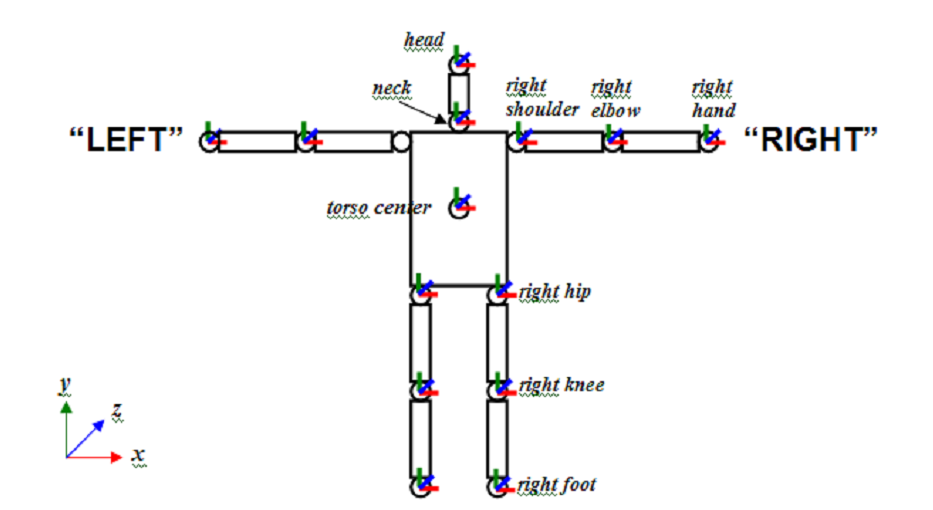
\includegraphics[width=0.9\columnwidth]{./figures/nite_joints.png}
	\end{center}
	\caption{Human Joints provided by NITE \cite{PS2102}}
	\label{fig:nite_joints}
\end{figure}


For a realistic simulation, collision spheres must be as large as possible without intersecting the skin mesh of the avatar. The optimal sphere fitting algorithm to satisfy this requirement is the straight forward approach to start with an infinitely small circle and expand it discretely until it intersects with the body contour: 
\begin{enumerate}
\item Take vector $J_i$ which represents the coordinates of the $i^{th}$
joint.
Initialize the radius of the sphere by setting it to the z-distance with the overlapping point in the depth map.
\begin{equation}
r_i^z=J_i^z-D^z(J_i^x,J_i^y)
\label{eqn:z_sphere_radius}
\end{equation}
\item Start with an infinitely small line segment parallel with x-axis. Expand it until it intersects with the body contour. Take the x-distance between the intersection point and the joint location. Repeat the same process with a line segment parallel with y-axis. Take the bigger radius. While expanding the segment, stop expanding and discard the corresponding result if the end of depth map is reach.
\begin{equation}
r_i^{x,y}=max(\| \pm J_i^{x,y} \mp D^{x,y}(J_i^{y,x},J_i^z)\|)
\label{eqn:x_y_sphere_radius}
\end{equation}
\item Take the minimum of three-axis differences, as there should be no intersection with the body contour and the shape must be a sphere.
\begin{equation}
r_i=min(r_i^{x,y,z})
\label{eqn:minimum_sphere-radius}
\end{equation}
\end{enumerate}

The process pseudocode is given in Algorithm \ref{algo:sphere_fitting}.

\begin{algorithm}
\dontprintsemicolon % Some LaTeX compilers require you to use \dontprintsemicolon instead
\KwIn{Optimized Depth Stream From Kinect}
\KwOut{Collision Sphere radii for each joint }
\ForEach{joint }{
$p=pos_{J_m}$\;
$r_z=\sqrt{P_z^2-D_z(P_x,P_y)^2}$
\For{i \bf{from} $P_x$ \bf{to} $0$ }{
\If{$D(i,P_y)$ \bf{equals}  $P_z$} {
  $r_x^- = i$\;
  break\;
 }
}
\For{i \bf{from} $P_x$ \bf{to} $depth_width$ }{
\If{$D(i,P_y)$ \bf{equals}  $P_z$} {
  $r_x^+ = i$\;
  break\;
 }
}
\For{j \bf{from} $P_y$ \bf{to} $0$ }{
\If{$D(P_x,j)$ \bf{equals}  $P_z$} {
  $r_y^- = j$\;
  break\;
 }
}
\For{j \bf{from} $P_y$ \bf{to} $depth_height$ }{
\If{$D(P_x,j)$ \bf{equals}  $P_z$} {
  $r_y^+ = j$\;
  break\;
 }
}
$r_m=min(r_z,r_x^-,r_x^+,r_y^-,r_y^+)$
}
\Return $(r_0,r_1 \ldots r_n)$ 
\caption{Sphere Fitting Algorithm}
\label{algo:sphere_fitting}
\end{algorithm}  

\subsubsection{Height and Width Parameters}

The width and height of the subject is important for determining the proper actual size for the cloth. However, a straightforward estimation of body height and shoulder width is prone to errors due to the noise and quality of the incoming depth map. In order to minimize the error factor, a larger of the subject's body are measured, to be used in width-height estimation later. This set of dimensions are listed in Table \ref{tbl:human_body_proportions}. 
For the sake of relative representation, head width and head height are taken as unit width and height respectively. The Measure Source column in the table denotes the source for the estimation of respective parameter:
\begin{itemize} 
\item
Joint location represents that the measurement will take the input subject joint locations as the reference.
\item 
Depth map represents the measurement will instead perform measurements based on the pixel distribution in the optimized subject depth map. 
\end{itemize}
They are often used together for better performance. Please note that some of these dimensions are not standard enough to be used as relative references, i.e. hip width, these parameters do not effect others in estimation process, and vica versa.

\begin{table}

\begin{tabularx}{\columnwidth}{ | p{0.2\columnwidth} |  p{0.2\columnwidth} | p{0.2\columnwidth} |  p{0.2\columnwidth} |}
\hline
\textbf{Distance} & \textbf{Width} & \textbf{Height} & \textbf{Measure Source} \\ \hline
Head & 1w (1) & 1h (2) & Depth Map+Joint Location \\ \hline
Body Height & - & 7 (3) & Depth Map \\ \hline
Hip Height & - & 4 (4) & Joint Location \\ \hline
Elbow-Fingertip & - & 2 (5) & Depth Map+Joint Location \\ \hline
Wrist to Fingertip & - & 1 (6) & Depth Map+Joint Location \\ \hline
Shoulder Width & 3 (7) & - & Depth Map+Joint Location \\ \hline
Hip Width & - (8) & - & Depth Map \\ \hline
Torso Height & - & - (9) & Joint Location \\ 
\hline
\end{tabularx}
\caption{Human Body Proportions \cite{Willis2012}. Numbers in parenthesis represent the lines on Figure \ref{fig:body_proportions}.}
\label{tbl:human_body_proportions}
\end{table}


\begin{figure}
	\begin{center}
			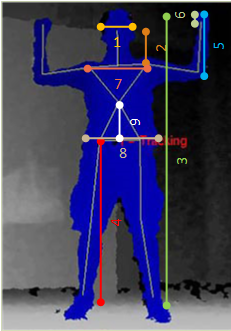
\includegraphics[width=0.9\columnwidth]{./figures/body_proportions.png}
	\end{center}
	\caption{Proportions on the Body}
	\label{fig:body_proportions}
\end{figure}

Measurements will be performed in real-world space rather than projective space as a real size estimation is crucial for determining the appropriate cloth size. Although the latter would be sufficient enough for simulation purposes only, when there is no concern of real-life apparel fitting. After the acquisition of the required scaling parameters for the subject, whole cloth and avatar should be scaled in three dimensions uniformly, in contrast with a segmented scaling. This decision is based on the scope of this work, as it is a standard-sized apparel fitting application, without extensive customization. Following the measurements, the body width and shoulder height are estimated as following:

\begin{enumerate}
\item Take the primary dimension (either body height or shoulder width) $P_i^0$. This process will be repeated for width (W) and height (H).
\item Using the remaining measurements in the set, estimate the primary dimension $P_i$ as $P_i^j$ using proportion $R_i^j$ from \ref{tbl:human_body_proportions}.
\begin{equation}
W,H_i^j=W,H_j \times R_i^j
\label{eqn:proportion_estimation}
\end{equation}
\item Find the optimized primary dimension as the mean of all estimations:
\begin{equation}
W,H_i=1/(n+1) \times \sum\limits_{j=0}^n W,H_i^j
\label{eqn:optimized_parameter}
\end{equation}
\end{enumerate}

\begin{algorithm}
\dontprintsemicolon % Some LaTeX compilers require you to use \dontprintsemicolon instead

$t_{proportion}=import(Table \ref{tbl:human_body_proportions})$ \;
$t_{primary}=w_{shoulder},h_{body}$ \;
$ct=cloth_{type}$\;
$width_{main}=t_{proportion}.width(ct)$\;
$width_{sum}=0$\;
$count_{effector}=0$\;
\ForEach{width \bf{in} $t_{proportion}$ }{
$w_i=measure(p_i)$\;
$w_i^j=w \times t_{proportion}.ratio(p_i,parameter_{main})$\;
$width_{sum}=width_{sum}+w_i^j $\;
$count_effector++ $\;
}
$width_{weighted}=width_{sum}/count_effector$
$x_s=width_{weighted}/width_{cloth}$\;

$height_{main}=t_{proportion}.height(ct)$\;
$height_{sum}=0$\;
$count_{effector}=0$\;
\ForEach{height \bf{in} $t_{proportion}$ }{
$h_i=measure(p_i)$\;
$h_i^j=h \times t_{proportion}.ratio(p_i,parameter_{main})$\;
$height_{sum}=height_{sum}+h_i^j $\;
$count_effector++ $\;
}
$height_{weighted}=height_{sum}/count_effector$
$y_s=height_{weighted}/height_{cloth}$\;
\Return{$(x_s,y_s)$}
\caption{Body Dimension Estimation}
\label{algo:cloth_resize}
\end{algorithm}

\subsection{Temporal Optimization}
\label{subsec:3.3} 

By now, we have acquired the required body dimensions and collision sphere parameters for a realistic simulation. 

Yet, the measurements are performed on a filtered version of a depth sensor with high error rates. In order to overcome the noise and overall depth-sense faults,
the prior measurements are repeated for the duration of 1 second, which corresponds to 30 frames of input depth map. 
A considerable different approach here would be to employ the temporal optimization on the depth map instead of the measured parameters. We realized the results suffer due to the motions of the subject, as most subjects failed to keep their exact form for one seconds.

Temporal averaging consists of collecting the specified parameters for each frame in one second and taking the mean. This step finalizes the parameters and delivers the required parameters for simulation environment creation. 
\begin{algorithm}
\dontprintsemicolon % Some LaTeX compilers require you to use \dontprintsemicolon instead
\KwIn{Raw Depth Stream From Kinect}
\KwOut{Depth Stream With Patched Holes and Gaussian Optimization }
$s=2 \times 30 Array for x and y scaling parameters for 30 frames$ \;
$r=16 \times 30 Array for joint radii for 30 frames$\;
\For{i \bf{from} 0 \bf{to} $30 frames$ }{
	r[i]=fitSpheres()\;
	s[i]=optimizeScaleParameters()\;
}
$r_{final}$=avg(r)\;
$s_{final}$=avg(s)\;
\caption{Temporal Averaging}
\label{algo:temporal_averaging}
\end{algorithm}


\section{Experiments}
\label{sec:4}
The optimization algorithm described in Section \ref{sec:4} is implemented on a virtual dressing framework, which provides a set of boiler plate features. These features are out of the scope of this work, the framework provides the testbench for experimentation. Boiler plate features are:
\begin{itemize}
  \item 3D Scene Rendering and Render Cycle Management
  \item Cloth Simulation Framework
  \item Depth Sensor Integration
\end{itemize} 
Optimization process runs after a subject is recognized, identified and calibrated for tracking. Following the parameter estimation, virtual avatar and cloth are created and simulation is started.

Table \ref{tbl:body_results} holds the measurements for the body dimensions, as well as the errors and the standart deviation of the measurements in 30 frames.  

\begin{table}
\begin{tabularx}{\columnwidth}{ | p{0.05\columnwidth} |   p{0.05\columnwidth} |   p{0.07\columnwidth} |   p{0.05\columnwidth}|   p{0.06\columnwidth}|   p{0.05\columnwidth}|   p{0.07\columnwidth}|   p{0.06\columnwidth}|   p{0.06\columnwidth} |}
\hline
  & \multicolumn{4}{c|}{\textbf{Shoulder Width (cm)}} & \multicolumn{4}{c|}{\textbf{Body Height (cm)}} \\ \hline
  \rotatebox{90}{Subject } & \rotatebox{90}{Real } & \rotatebox{90}{Estimated } & \rotatebox{90}{Error } & \rotatebox{90}{Deviation } & \rotatebox{90}{Real } & \rotatebox{90}{Estimated } & \rotatebox{90}{Error } & \rotatebox{90}{Deviation } \\ \hline
 1 & 43 & 43.6 & 1\% & 7.8 & 172 & 170.8 & 0.6\% & 8.5  \\ \hline
\end{tabularx}
\caption{Body Size Estimations and Errors}
\label{tbl:body_results}
\end{table}

The total time for the optimization algorithm did not exceed 1.005 seconds in any of the cases. Considering 1.0 seconds is the time for acquiring 30 frames of input from the depth sensor, it is safe to say that the proposed algorithm does not introduce any delays and problems for a real time application, as it needs to run only once in the beginning of the simulation.

For the collision spheres, the quality of the result can be assessed by the smoothness of the collision simulation, as seen in Figure \ref{fig:system}. Throughout the program, no unnatural intersection between the cloth the avatar took place, while the cloth appears to rest on the skin naturally, without space between two meshes.

\begin{figure}
	\begin{center}
			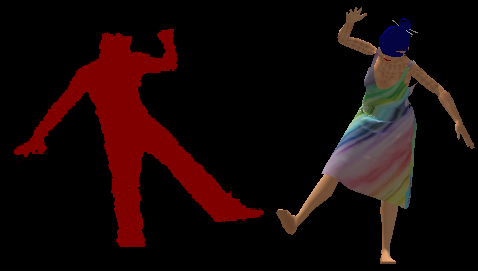
\includegraphics[width=0.9\columnwidth]{./figures/scshot.png}
	\end{center}
	\caption{System At Work}
	\label{fig:system}
\end{figure}

\section{Conclusion and Future Work}
\label{sec:5}
The simulation framework is shown in Figure \ref{fig:system}. Both optimization and the simulation are performed on a high-end PC with Intel i7- and NVIDIA GeForce GTX560Ti. The maximum optimization time is 1.002 seconds, which is constrained by the frame rate of the depth sensor. The actual simulation runs at 600fps on 1920x1080 resolution. Body sizes are estimated with error rates less than 5\%, which is sufficient for the realism of the simulation and determining the appropriate apparel size. 

In future work, we would like to improve the quality of measurements by using data from the RGB sensor as well, as it provides valuable information. We would also like to provide more collision sphere information to the framework for better collision detection.

 
\begin{thebibliography}{}

\bibitem{PS2102}
PrimeSense, NITE,  PrimeSense Natural Interaction (2012)

\bibitem{Willis2012}
Willis B,  Body Proportions in Art,  [Online] (2012)

\bibitem{Microsoft2013}
Microsoft,  Kinect for Windows, [Online] (2013)

\bibitem{OpenNI2013}
OpenNI,  The standard framework for 3D sensing, [Online] (2013)

\bibitem{Peter2012}
Peter Henry and Michael Krainin and Evan Herbst and Xiaofeng Ren and Dieter Fox, RGB-D mapping: Using Kinect-style depth cameras for dense 3D modeling of indoor environments, The International Journal of Robotics Research , Volume 31, 647-663 (2012)

\bibitem{Gallo2012}
Gallo L,  Controller-free exploration of medical image data: Experiencing the Kinect, Computer Based Medical Systems ,Volume 24,  (2011)

\bibitem{Giovanni2012}
Stevie Giovanni, Yeun Chul Choi, Jay Huang, Khoo Eng Tat, and KangKang Yin,  Virtual Try-On Using Kinect and HD Camera, Lecture Notes in Computer Science , Volume 7660, 55-65 , (2012)

\bibitem{Yao2011}
Yao-Jen Changa and Shu-Fang Chenb and Jun-Da Huang,  A Kinect-based system for physical rehabilitation: A pilot study for young adults with motor disabilities, Research in Developmental Disabilities, Volume 32, 2566�2570 (2011)

\bibitem{Protopsaltou2002}
D. Protopsaltou, C. Luible, M. Arevalo-Poizat, N. Magnenat-Thalmann, A body and garment creation method for an Internet based virtual fitting room. Proc. Computer Graphics International 2002 (CGI '02), Springer, pp. 105-122, 2002.
 
\bibitem{Zhang2008}
Wei Zhang, Takashi Matsumoto, Juan Liu, Maurice Chu, and Bo Begole. An intelligent fitting room using multi-camera perception. In Proceedings of the 13th international conference on Intelligent user interfaces (IUI '08). ACM, New York, NY, USA, 60-69, 2008 

\bibitem{Cheung2005}
Kong-man Cheung, Simon Baker, Takeo Kanade,Shape-From-Silhouette Across Time Part II: Applications to Human Modeling and Markerless Motion Tracking,International Journal of Computer Vision ,Volume 63, pp 225-245, 2005

\bibitem{Khoshelham2012}
Khoshelham, K.; Elberink, S.O. Accuracy and Resolution of Kinect Depth Data for Indoor Mapping Applications. Sensors 2012, 12, 1437-1454.

\bibitem{Matyunin2011}
Matyunin, S.; Vatolin, D.; Berdnikov, Y.; Smirnov, M.; , "Temporal filtering for depth maps generated by Kinect depth camera," 3DTV Conference: The True Vision - Capture, Transmission and Display of 3D Video (3DTV-CON), 2011 , vol., no., pp.1-4, 16-18 May 2011

\bibitem{Breyer2012}
Breyer, M,  25 Shocking Fashion Industry Statistics, [Online] (2012)

\bibitem{Fredricksen2012}
Fredricksen C,Apparel Drives US Retail Ecommerce Sales Growth, [Online] (2012) 

\bibitem{Fitnect2012}
Fitnect Interactive,Fitnect, [Online] (2012)

\bibitem{Styku2013}
Styku, LLC, [Online] (2013)

\bibitem{FaceCake2013}
FaceCake Marketing Technologies Inc, [Online] (2013)

\end{thebibliography}

\end{document}



